\documentclass[a4paper]{article}

\usepackage[utf8]{inputenc}
\usepackage[english]{babel}
\usepackage{graphics}
\usepackage{caption}
\usepackage{subcaption}
\usepackage[demo]{graphicx}
\usepackage{enumitem}
\usepackage{longtable}
\usepackage{listings}
\usepackage{listingsutf8}
\usepackage{framed}
\usepackage{float}
\usepackage{hyperref}
\usepackage{amsmath}

\begin{document}

\begin{titlepage}

\begin{center}
\vspace*{-1in}
\begin{figure}[htb]
\begin{center}

\includegraphics[width=8cm]{logoUZ.png}
\end{center}
\end{figure}

\vspace*{0.3in}

UNIVERSIDAD DE ZARAGOZA \\

\vspace*{0.3in}

\begin{large}
SISTEMAS Y TECNOLOGÍAS WEB\\
\end{large}
\vspace*{0.2in}
\begin{Large}
\textbf{FelinoTweets} \\
\end{Large}
\vspace*{0.3in}
\begin{large}
\end{large}
\vspace*{0.5in}
\rule{80mm}{0.1mm}\\
\vspace*{0.1in}
\begin{large}
Autores: \\
Alejandro Márquez Ferrer (NIP: 566400)\\
Jaime Ruiz-Borau Vizárraga (NIP: 546751)\\
Alejandro Royo Amondarain (NIP: 560285)\\

\end{large}
\end{center}

\end{titlepage}
\tableofcontents

\newpage
\section{Resumen}

	\paragraph{} El trabajo propuesto tiene como objetivo el desarrollo de un sistema que permita gestionar, mediante una interfaz típica de control de acceso de usuarios, una o varias cuentas de \textit{Twitter}.

\section{Propuestas similares - Hootsuite}

	\paragraph{} Se ha analizado principalmente un servicio web similar a la propuesta, \textit{Hootsuite}. Esta herramienta ofrece en su vista principal un panel de control (\textit{dashboard}) para gestionar las cuentas de diferentes redes sociales (\textit{Twitter}, \textit{Facebook}...). Es posible añadir nuevas columnas o eliminarlas para estar al tanto de la mayor cantidad de información posible. 
	
	\paragraph{} Se proporcionan varias versiones de esta aplicación, una gratuita (con funcionalidades limitadas) y otra de pago que ofrece al usuario servicios adicionales como el de realizar informes de estadísticas sobre sus redes sociales.

\section{Arquitectura de alto nivel}
	\paragraph{} A continuación se presenta un diagrama arquitectural de alto nivel con la estructura de la aplicación desarrollada, seguido de una descripción más en detalle de cada una de las partes que la componen:
	\begin{figure}[H]
		\centering
		\includegraphics[width=260px]{diagarq.png}
		\caption{Diagrama arquitectural de alto nivel}
		\label{fig:diagarq}
	\end{figure}
	\newpage
	\subsection{Componentes}
		\begin{itemize}
			\item \textbf{Twitter:} Este componente se encarga de todas las interacciones con Twitter según las solicitudes del Cliente o de otros componentes del servidor. Devuelve y publica tweets y permite realizar retweets o dar "Me gusta".
			\item \textbf{Stats:} Gestiona todas las estadísticas, tanto de usuarios como del administrador del sistema. Se comunica con la base de datos en mLab y con el componente Twitter de FelinoTweets para elaborar las estadísticas.
			\item \textbf{URLs:} Es el componente encargado de acortar urls para publicarlas en los tweets enviados a través de la aplicación. Se comunica con la base de datos para almacenar el usuario que acortó una cierta url, la url acortada y el número de clicks realizados sobre dicha url.
			\item \textbf{Users:} Componente que gestiona los usuarios de la aplicacion de Felino Tweets. Se comunica con la base de datos para obtener información de los usuarios, así como realizar tareas de registro y login.
			\item \textbf{Twitter Accounts:} Por último, este componente gestiona toda la información asociada a cuentas de Twitter, así como sus tokens para poder publicar tweets y recibir información de Twitter.
		\end{itemize}
		\paragraph{} La descripción detallada de cada función del API se encuentra en el apartado \textbf{API}.

\section{Modelo de datos}

	\paragraph{} Se han definido varias colecciones para almacenar la información de los disintos usuarios de la aplicación, de sus cuentas de twitter, de los enlaces a acortar o para almacenar estadísticas que proporcionan a los usuarios, ya sean administradores o usuarios normales una retroalimentación de su interacción con la aplicación. A continuación se describen todas las colecciones utilizadas:
	
	\begin{itemize}
	\item \textbf{hashtag}: contiene la información almacenada sobre cada \textit{hashtag}.
		
		\begin{itemize}
		\item user\_id : String,
		\item account\_id : String,
		\item hashtag : String
		\end{itemize}
		
	\item \textbf{registrations}: almacena la información relativa a los diferentes eventos de acceso que pueden tener lugar: \textit{alta}, \textit{baja} y \textit{acceso}. Asociada a cada evento se guarda también la fecha, de esta forma se puede utilizar esta colección para crear estadísticas al respecto.
		
		\begin{itemize}
		\item type : String,
		\item date : Date
		\end{itemize}
	 
	\item \textbf{scheduled\_tweets}: contiene toda la información necesaria para representar un \textit{tweet}.
	
		\begin{itemize}
		\item user\_id : String,
		\item account\_id : String,
		\item date : Date,
		\item text : String
		\end{itemize}
	
	\item \textbf{twitter\_accounts}: guarda la información relativa a la asociación entre una cuenta de \textit{twitter} y una cuenta de usuario de la aplicación, así como los tokens necesarios para comunicarse con el \textbf{API} de \textit{Twitter}.
	
		\begin{itemize}
		\item account\_id : String,
		\item token : String,
		\item token\_secret : String,
		\item profile\_name : String,
		\item photo\_url : String,
		\item description : String,
		\end{itemize}
	
	\item \textbf{url}: contiene la asociación entre \textit{urls} acortadas y \textit{urls} originales para poder realizar la redirección.
	
		\begin{itemize}
		\item short\_url : String,
		\item long\_url : String,
		\item user\_id : String,
		\item clicks : Number
		\end{itemize}
	
	\item \textbf{user}: almacena toda la información relativa a un usuario de la aplicación. Se guardan tanto datos personales como fechas de acceso y registro o número total de tweets enviado (representan la suma de tweets enviados por todas las cuentas de \textit{twitter} asociadas a dicho usuario).
	
		\begin{itemize}
		\item admin : Boolean,
		\item email : String,
		\item password : String,
		\item first\_name : String,
		\item last\_name : String,
		\item registration\_date : Date,
		\item last\_access\_date : Date,
		\item n\_tweets : Number		
		\end{itemize}
	
	\end{itemize}

\newpage
\section{API REST}

	\paragraph{} En este apartado se recogen todos los endpoints de cada componente del API desarrollados, junto a una descriptición de lo que hace, sus parámetros y ejemplos de uso.
	
	\subsection{API del componente Twitter}
	
	\subsection{API del componente Stats}
	
	\subsection{API del componente URLs}
	app.get('/url', findAllUrls);
	app.get('/url/:shorturl', findById);
	app.post('/url', addUrl);
	app.delete('/url', deleteAllUrls);
	app.delete('/url/:shorturl',deleteUrl);
	\begin{itemize}
		\item \textbf{GET /url:} Devuelve una lista con todas las URLs acortadas de la base de datos.
	\end{itemize}
	
	\subsection{API del componente Users}
	
	\subsection{API del componente Twitter accounts}
\section{Analíticas}

	\paragraph{} Se ha desarrollado un servicio de analíticas que ofrece datos acerca del comportamiento del conjunto de usuarios de la aplicación para un usuario de tipo administrador. Por otro lado, el mismo servicio ofrece estadísticas acerca de las cuentas de \textit{Twitter} asociadas con un usuario.
	
	\subsection{Analíticas de administrador}
	
		\paragraph{} El objetivo de estas estadísticas es el de dar al administrador una visión del modo en que sus usuarios utilizan la aplicación. A continuación se muestran las gráficas que puede visualizar el administrador del sistema:
		
			\begin{figure}[H]
				\centering
				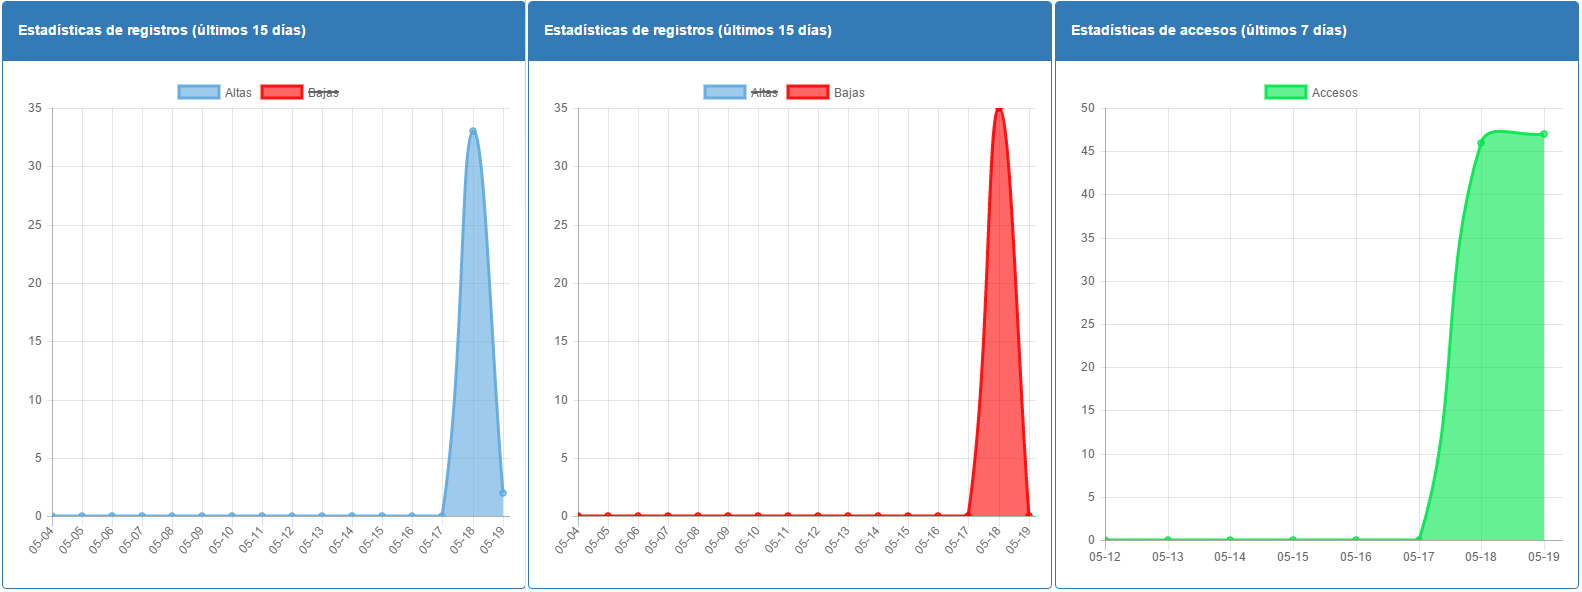
\includegraphics[width=1\linewidth]{img/altas-bajas-accesos}
				\caption{Registros, cuentas borradas en la aplicación en los útlimos 15 días y accesos de los usuarios (no únicos) a la apliación en los últimos 7 días.}
				\label{fig:altas-bajas-accesos}
			\end{figure}
			
			\begin{figure}[H]
				\centering
				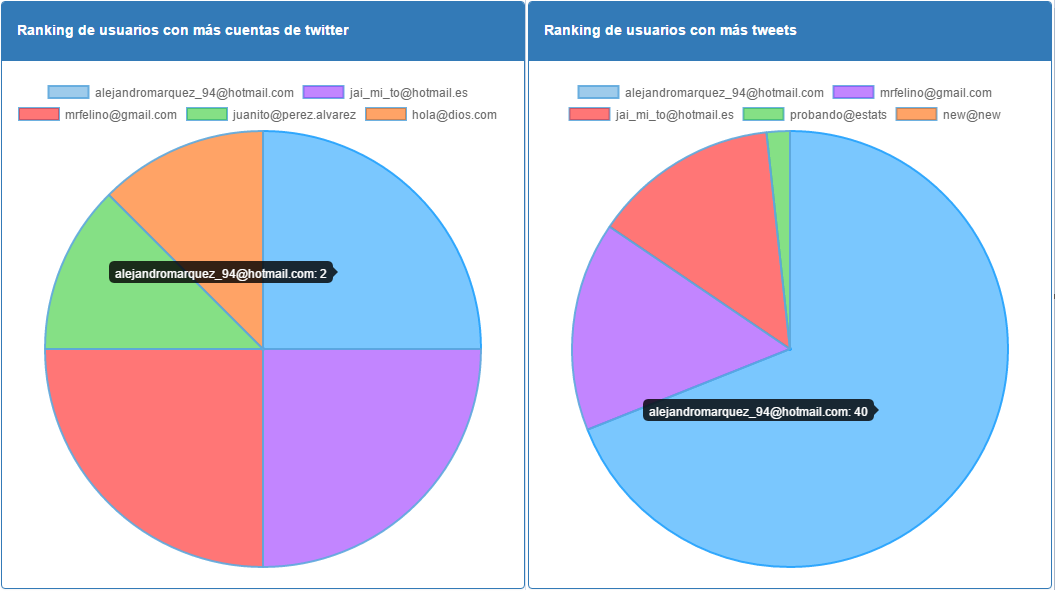
\includegraphics[width=1\linewidth]{img/rankingsAdmin}
				\caption{Ranking de cuentas con mayor número de tweets enviados (izquierda) y ranking de cuentas de la aplicación con mayor número de cuentas de twitter asociadas cada una (derecha).}
				\label{fig:rankingsAdmin}
			\end{figure}
	
	\subsection{Analíticas de usuario} 

		\paragraph{} El interés de estas gráficas para el usuario reside en informarle de la diferente repercursión que tienen sus disintas cuentas de \textit{Twitter} asociadas.

\section{Implementación}

\section{Modelo de navegación}

\section{Despliegue del sistema (instrucciones)}

\section{Validación (test, pruebas realizadas)}

\section{Análisis de problemas}

\section{Distribución de tiempos}
	\subsection{Diagrama de Gannt}
	\subsection{Horas de esfuerzo del equipo y por separado en tareas}

\section{Conclusiones}
	\subsection{Conclusiones del proyecto}
	\subsection{Valoración personal del grupo}
	\subsection{Valoración personal de cada miembro}
\section{Anexos}

\newpage
\begin{thebibliography}{99} 
\bibitem{paraQueSirve} \textbf{Title} - Consulted in XXXXX aaaa. [\url{link}]

\end{thebibliography}

\end{document}